\documentclass[tikz,border=8pt]{standalone}
\usepackage{tikz}
\usetikzlibrary{positioning,arrows.meta,calc}

\begin{document}
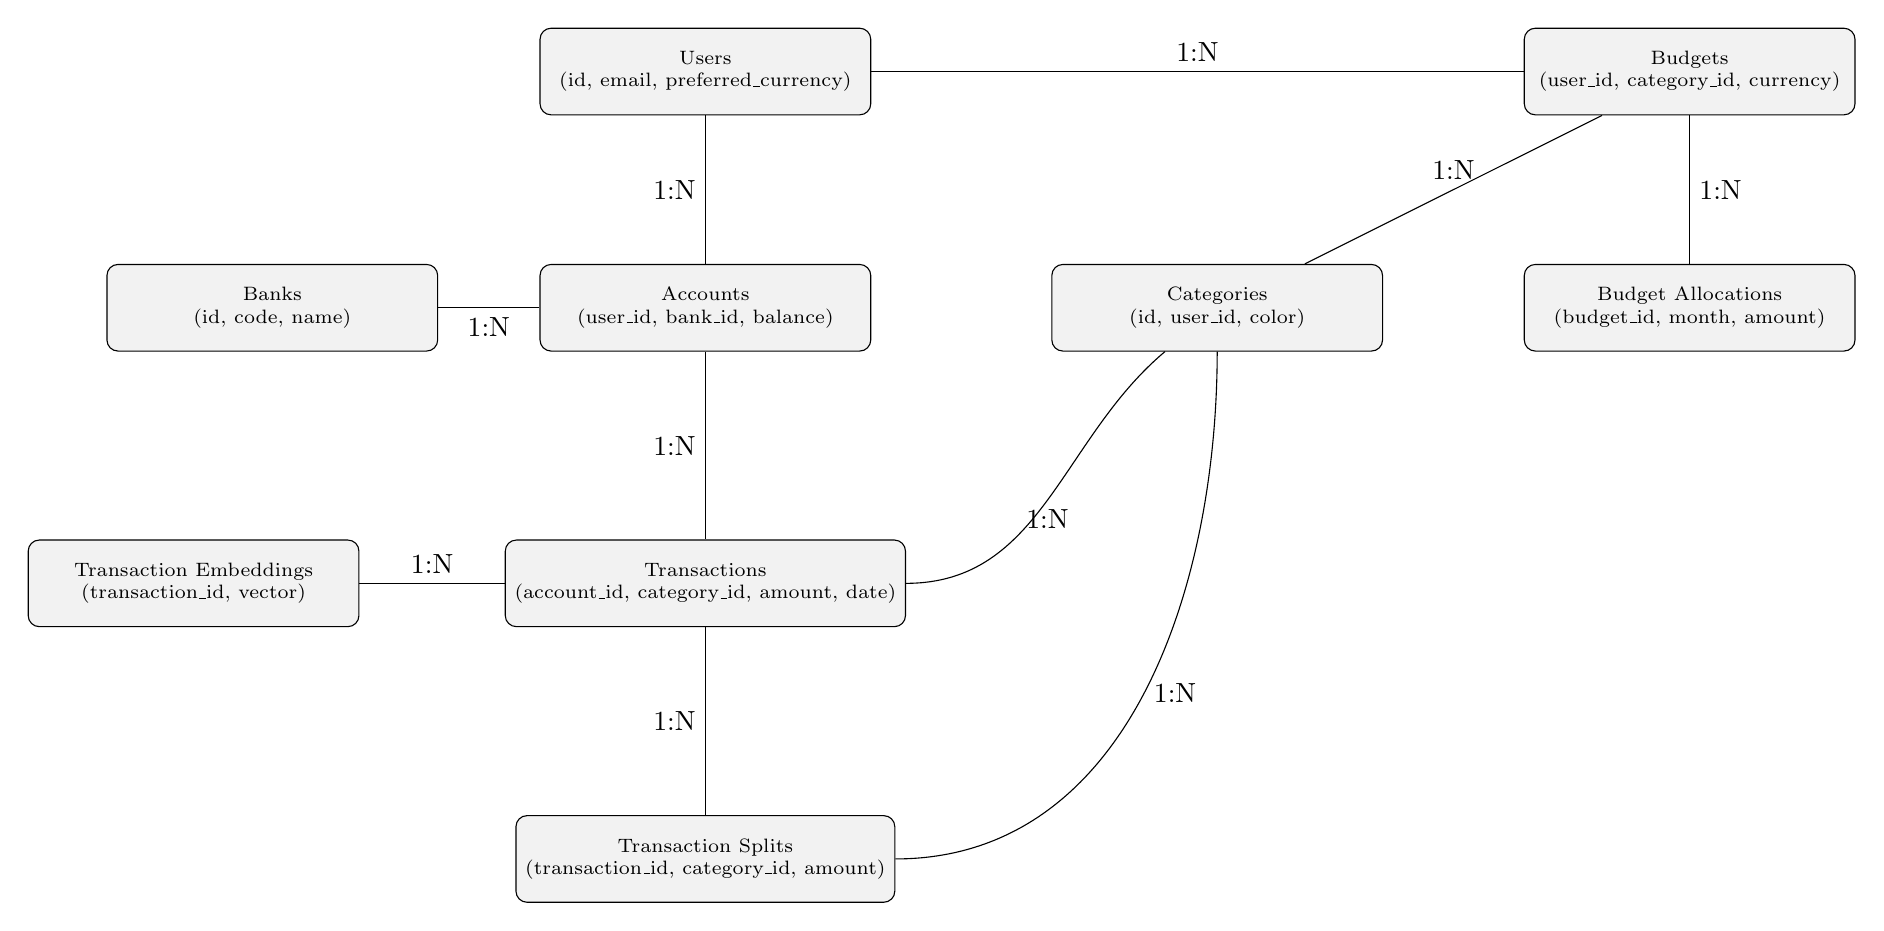
\begin{tikzpicture}[
    table/.style={
        draw,
        rounded corners,
        fill=gray!10,
        minimum width=4.2cm,
        minimum height=1.1cm,
        font=\scriptsize,
        align=center
    },
    every edge/.style={->, very thick, >=Stealth}
]
    \node (users) at (0,1.5) [table] {Users\\(id, email, preferred\_currency)};
    \node (banks) at (-5.5,-1.5) [table] {Banks\\(id, code, name)};
    \node (accounts) at (0,-1.5) [table] {Accounts\\(user\_id, bank\_id, balance)};
    \node (transactions) at (0,-5.0) [table] {Transactions\\(account\_id, category\_id, amount, date)};
    \node (splits) at (0,-8.5) [table] {Transaction Splits\\(transaction\_id, category\_id, amount)};

    \node (categories) at (6.5,-1.5) [table] {Categories\\(id, user\_id, color)};
    \node (embeddings) at (-6.5,-5.0) [table] {Transaction Embeddings\\(transaction\_id, vector)};
    \node (budgets) at (12.5,1.5) [table] {Budgets\\(user\_id, category\_id, currency)};
    \node (allocations) at (12.5,-1.5) [table] {Budget Allocations\\(budget\_id, month, amount)};

    \draw (users) -- node[midway,left]{1:N} (accounts);
    \draw (banks) -- node[midway,below]{1:N} (accounts);
    \draw (accounts) -- node[midway,left]{1:N} (transactions);
    \draw (transactions) -- node[midway,left]{1:N} (splits);
    \draw (transactions) -- node[midway,above]{1:N} (embeddings);

    \draw (users) -- node[midway,above]{1:N} (budgets);
    \draw (categories) -- node[midway,above]{1:N} (budgets);
    \draw (budgets) -- node[midway,right]{1:N} (allocations);

    \draw (categories) to[out=-140,in=0] node[midway,below]{1:N} (transactions);
    \draw (categories) to[out=-90,in=0] node[midway,right]{1:N} (splits);
\end{tikzpicture}
\end{document}
